\documentclass{standalone}
\usepackage{tikz}
\usetikzlibrary{calc, decorations, fit, shapes}

\usepackage{soul}
\usepackage{xcolor}
\definecolor{morange}{RGB}{255,127,14}
\definecolor{mblue}{RGB}{31,119,180}
\definecolor{mred}{RGB}{214,39,40}
\definecolor{mpurple}{RGB}{148,103,189}
\definecolor{mgreen}{RGB}{44,160,44}

\newcommand\ppbb{path picture bounding box}

\begin{document}
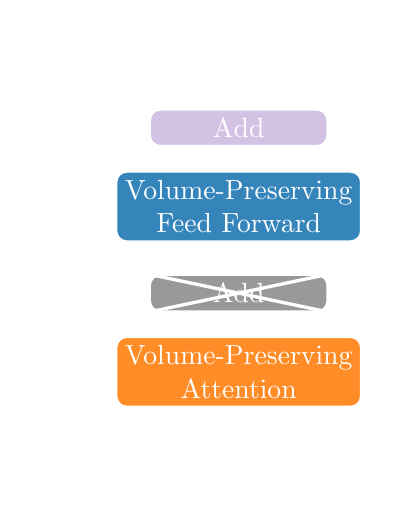
\begin{tikzpicture}[module/.style={draw, very thick, rounded corners, minimum width=15ex},
    attmodule/.style={module, fill=morange!90},
    ffnnmodule/.style={module, fill=mblue!90},
    addmodule1/.style={module, fill=black!40,
                     path picture={\draw (\ppbb.north west) -- (\ppbb.south east)
                                         (\ppbb.south west) -- (\ppbb.north east);
                                         } % <---
                      },
    addmodule2/.style={module, fill=mpurple!40},
    crossout/.style = {draw, inner sep=0pt, cross out, fit=#1},
    arrow/.style={-stealth, thick, rounded corners},
    color = white,
]
\node (input) {Input};
\node[above of=input, attmodule, align=center, yshift=.3cm] (att) {Volume-Preserving\\Attention};
\node[above of=att, addmodule1, align=center] (add1) {Add};
\node[above of=add1, ffnnmodule, align=center, yshift=.1cm] (ffnn) {Volume-Preserving\\Feed Forward};
\node[above of=ffnn, addmodule2, align=center] (add2) {Add};
\node[above of=add2] (output) {Output};

%\node[crossout=(addmodule1)] {};

\coordinate (attresidual) at ($(att.south)!0.5!(input.north)$);
\coordinate (ffnnresidual) at ($(ffnn.south)!0.5!(add1.north)$);
\coordinate[left of=add2, xshift=-.8cm] (leftofadd2);
\coordinate[left of=add1, xshift=-.8cm] (leftofadd1);

\node[fit=(attresidual)(att)(add2)(leftofadd2)(leftofadd1),draw, ultra thick, rounded corners, label=left:$\mathrm{L\times}$] (encoder) {};
%\draw[arrow, black!30] (attresidual)-|(leftofadd1)--(add1);
\draw[arrow] (ffnnresidual)-|(leftofadd2)--(add2);

\draw[arrow] (input) -- (att);
\draw[arrow] (att) -- (add1); 
\draw[arrow] (add1) -- (ffnn);
\draw[arrow] (ffnn) -- (add2); 
\draw[arrow] (add2) -- (output);

\end{tikzpicture}
\end{document}
